% THIS DOCUMENT IS FOLLOWS THE VOLERE TEMPLATE BY Suzanne Robertson and James Robertson
% ONLY THE SECTION HEADINGS ARE PROVIDED
%
% Initial draft from https://github.com/Dieblich/volere
%
% Risks are removed because they are covered by the Hazard Analysis
\documentclass[12pt]{article}

\usepackage{booktabs}
\usepackage{tabularx}
\usepackage{hyperref}
\hypersetup{
    bookmarks=true,         % show bookmarks bar?
      colorlinks=true,      % false: boxed links; true: colored links
    linkcolor=red,          % color of internal links (change box color with linkbordercolor)
    citecolor=green,        % color of links to bibliography
    filecolor=magenta,      % color of file links
    urlcolor=cyan           % color of external links
}
\usepackage{graphicx}
\graphicspath{ {./images/} } % relative path

\newcommand{\lips}{\textit{Insert your content here.}}

\input{../Comments}
\input{../Common}

\begin{document}

\title{Software Requirements Specification for \progname: subtitle describing software} 
\author{\authname}
\date{\today}
	
\maketitle

~\newpage

\pagenumbering{roman}

\tableofcontents

~\newpage

\section*{Revision History}

\begin{tabularx}{\textwidth}{p{3cm}p{2cm}X}
\toprule {\textbf{Date}} & {\textbf{Version}} & {\textbf{Notes}}\\
\midrule
Date 1 & 1.0 & Notes\\
Date 2 & 1.1 & Notes\\
\bottomrule
\end{tabularx}

~\\

~\newpage
\section{Purpose of the Project}
\subsection{User Business}
Music theory is challenging and intimidating to learn for beginners, 
however, the act of playing an instrument does not inherently require 
extensive theoretical knowledge. This project aims to bridge the gap 
between deep theoretical understanding and playing instruments. It 
shall aid musicians with limited music theory knowledge by translating 
analog instrument audio into sheet music and other applicable formats 
that users can use to visualize and document their music-making. The 
project also aims to foster ease of collaboration between musical 
artists for efficient communication. 
\subsection{Goals of the Project}
The goal of the project is to develop a fast, accurate sheet music generator 
paired with an intuitive, user-friendly interface that requires minimal effort 
to learn. If successful, it will encourage the proliferation of musical creativity 
among various audiences. This goal lends itself to several metrics, such as 
computational performance compared to existing products or its reach to certain 
demographics. Ultimately, the benefit of the project will be measured by the number 
of original pieces created.
\section{Stakeholders}
\subsection{Client}
\lips
\subsection{Customer}
\lips
\subsection{Other Stakeholders}
\lips
\subsection{Hands-On Users of the Project}
\lips
\subsection{Personas}
\lips
\subsection{Priorities Assigned to Users}
\lips
\subsection{User Participation}
\lips
\subsection{Maintenance Users and Service Technicians}
\lips

\section{Mandated Constraints}
\subsection{Solution Constraints}
\lips
\subsection{Implementation Environment of the Current System}
\lips
\subsection{Partner or Collaborative Applications}
\lips
\subsection{Off-the-Shelf Software}
\lips
\subsection{Anticipated Workplace Environment}
\lips
\subsection{Schedule Constraints}
\lips
\subsection{Budget Constraints}
\lips
\subsection{Enterprise Constraints}
\lips

\section{Naming Conventions and Terminology}
\subsection{Glossary of All Terms, Including Acronyms, Used by Stakeholders
involved in the Project}
\lips

\section{Relevant Facts And Assumptions}
\subsection{Relevant Facts}
\begin{itemize}
  \item This project is under irregular time constraints, given that it is 
  for an undergraduate-level software engineering course. 
  \item Digitizing and transcribing polyphonic audio from multiple instruments
   is a difficult task and may be unachievable due to the aforementioned time constraints. 
  \item Many products are currently available as alternatives to what this project hopes 
  to accomplish. The team will use these products and their functionalities as metrics for success.
\end{itemize}
\subsection{Business Rules}
\begin{enumerate}
  \item Instrument Support
  \begin{itemize}
    \item The application only supports a predefined list of instruments.
    \item No instruments may be added by the user to the predefined list.
  \end{itemize}
  \item Music Theory Compliance
  \begin{itemize}
    \item The application must generate score sheets that adhere to basic music 
    theory rules (e.g., correct note placement, no overlapping notes, etc.).
    \item The application must generate a score sheet within a reasonable amount of time
    to ensure a smooth user experience. 
  \end{itemize}
  \item Ownership
  \begin{itemize}
    \item The application must clearly identify and display the creator/owner of the score.
  \end{itemize}
\end{enumerate}
\subsection{Assumptions}
Assumptions are seperated into two categories based on the effect their falsehood will have 
on the application:
\begin{enumerate}
  \item Should the following assumptions be false, the application will be unusable:
  \begin{itemize}
    \item Users of the application have access to the hardware required, such as a music 
    interface or quality microphone.
    \item Users have access to a desktop or portable computer to use the application.
  \end{itemize}
  \item Should the following assumptions be false, the application will perform at sub-optimally: 
  \begin{itemize}
    \item The operational environment has low levels of background noise.
    \item The human voice is not considered an instrument that the application can handle input from.
    \item Users have a superficial level of understanding of music theory in order to understand 
    what the application does.
  \end{itemize}
\end{enumerate}

\section{The Scope of the Work}
\subsection{The Current Situation}
The following activity diagram illustrates the workflow of manual score sheet generation, the process
which the application intends to improve upon.\\\\
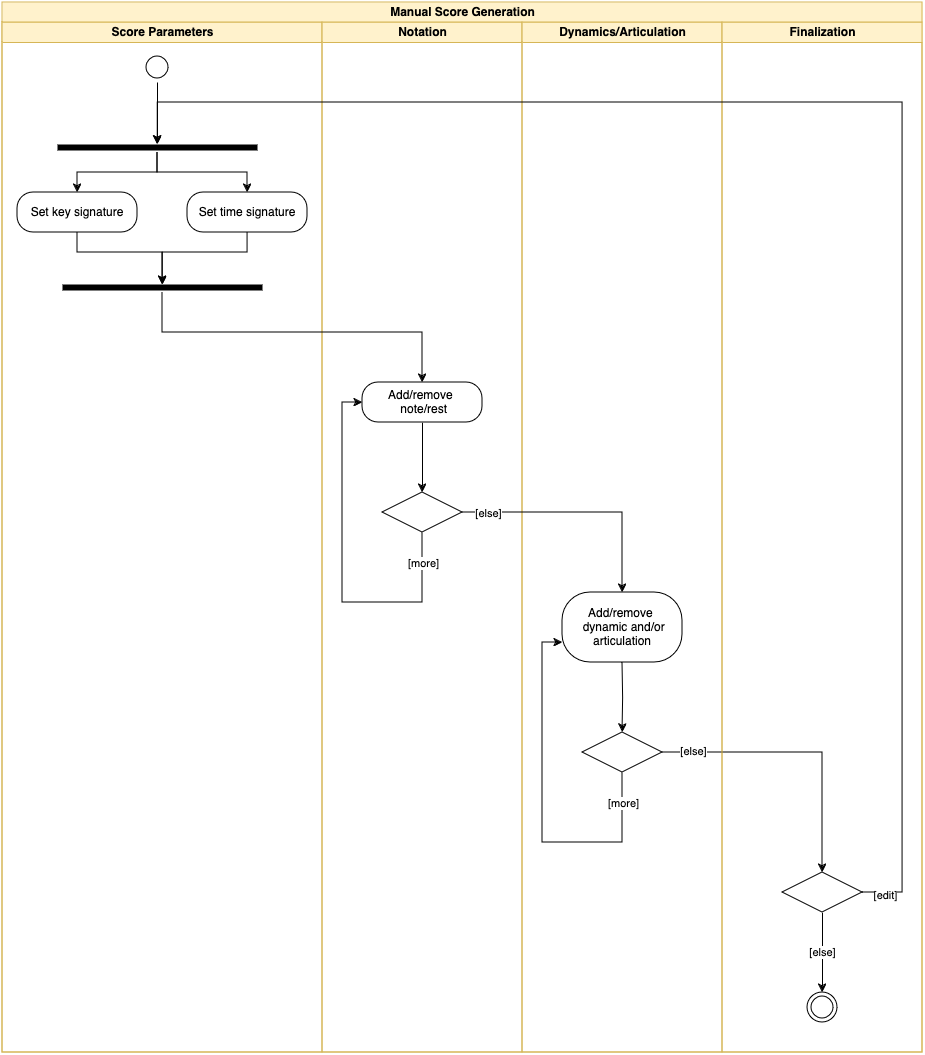
\includegraphics[width=\textwidth]{SRS-manual-score-process.png}
\subsection{The Context of the Work}
The diagram below shows the context in which the development of the application is taking place. It shows
adjacent systems and their associated inputs and outputs as it relates to the application and it's work. \\\\
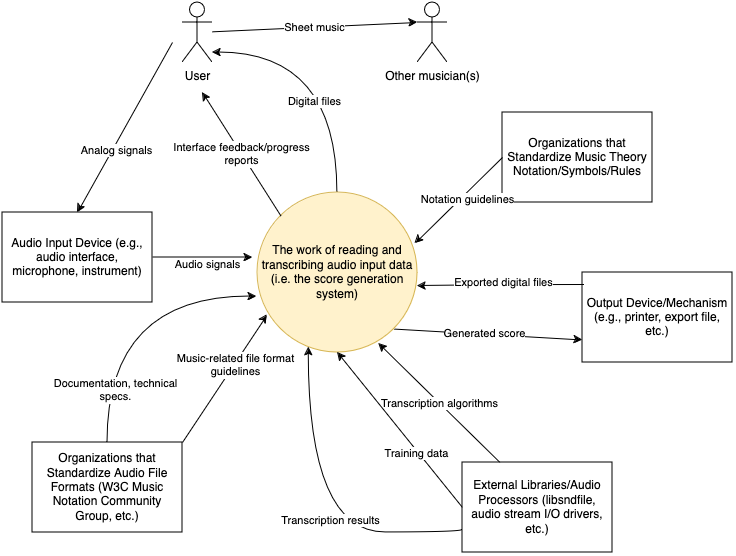
\includegraphics[width=\textwidth]{SRS-contex-diagram.png}

\subsection{Work Partitioning}
The table below summarizes the business events that might be triggered by adjacent organizations
or application users themselves.\\
\begingroup
\renewcommand{\arraystretch}{1.25}
\begin{tabular}{|>{\raggedright}p{3cm}|>{\raggedright}p{4.25cm}|>{\raggedright\arraybackslash}p{6cm}|}
  \hline
  EVENT NAME & INPUT/OUTPUT & SUMMARY OF BUC \\
  \hline
  BE1. User provides audio signals. & Audio signals (IN) & Digitize the input audio signals.\\
  \hline
  BE2. Audio transcription. & Transcription results (IN) & Record the notes transcribed. \\
  \hline
  BE3. Score completion. & Generated score (OUT) & Finalize the transcription results into proper music notation/symbols.\\
  \hline
  BE4. Export files. & Exported digital files (IN)  & Convert the generated score into a digital file format for export (see BE6.).\\
  \hline
  BE5. Progress reports. & Interface feedback/progress reports (OUT) & Provide visual indicators to user of transcription status.\\
  \hline
  BE6. Share sheet music. & Digital files (OUT)  & Output the exportable file format (see BE4.).\\
  \hline
\end{tabular}
\endgroup

\subsection{Specifying a Business Use Case (BUC)}
The use case diagram below has been used to specify the details of the BUC 
associated with BE1.\\
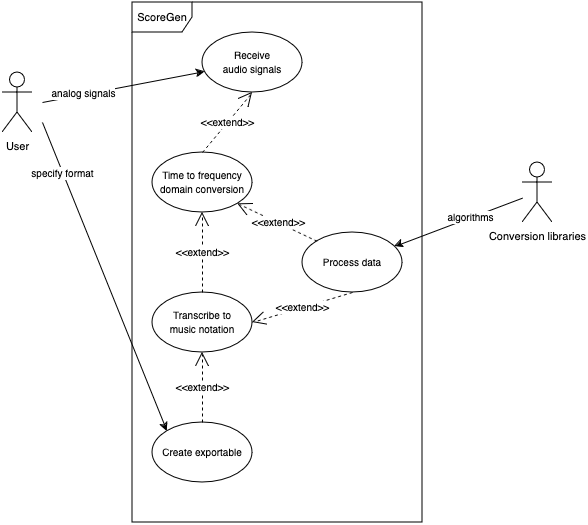
\includegraphics[width=\textwidth]{BUC.png}

\section{Business Data Model and Data Dictionary}
\subsection{Business Data Model}
\lips
\subsection{Data Dictionary}
\lips

\section{The Scope of the Product}
\subsection{Product Boundary}
\lips
\subsection{Product Use Case Table}
\lips
\subsection{Individual Product Use Cases (PUC's)}
\lips

\section{Functional Requirements}
\subsection{Functional Requirements}
\lips

\section{Look and Feel Requirements}
\subsection{Appearance Requirements}
\lips
\subsection{Style Requirements}
\lips

\section{Usability and Humanity Requirements}
\subsection{Ease of Use Requirements}
\lips
\subsection{Personalization and Internationalization Requirements}
\lips
\subsection{Learning Requirements}
\lips
\subsection{Understandability and Politeness Requirements}
\lips
\subsection{Accessibility Requirements}
\lips

\section{Performance Requirements}
\subsection{Speed and Latency Requirements}
\lips
\subsection{Safety-Critical Requirements}
\lips
\subsection{Precision or Accuracy Requirements}
\lips
\subsection{Robustness or Fault-Tolerance Requirements}
\lips
\subsection{Capacity Requirements}
\lips
\subsection{Scalability or Extensibility Requirements}
\lips
\subsection{Longevity Requirements}
\lips

\section{Operational and Environmental Requirements}
\subsection{Expected Physical Environment}
\lips
\subsection{Wider Environment Requirements}
\lips
\subsection{Requirements for Interfacing with Adjacent Systems}
\lips
\subsection{Productization Requirements}
\lips
\subsection{Release Requirements}
\lips

\section{Maintainability and Support Requirements}
\subsection{Maintenance Requirements}
\lips
\subsection{Supportability Requirements}
\lips
\subsection{Adaptability Requirements}
\lips

\section{Security Requirements}
\subsection{Access Requirements}
\lips
\subsection{Integrity Requirements}
\lips
\subsection{Privacy Requirements}
\lips
\subsection{Audit Requirements}
\lips
\subsection{Immunity Requirements}
\lips

\section{Cultural Requirements}
\subsection{Cultural Requirements}
\lips

\section{Compliance Requirements}
\subsection{Legal Requirements}
\lips
\subsection{Standards Compliance Requirements}
\lips

\section{Open Issues}
\lips

\section{Off-the-Shelf Solutions}
\subsection{Ready-Made Products}
\lips
\subsection{Reusable Components}
\lips
\subsection{Products That Can Be Copied}
\lips

\section{New Problems}
\subsection{Effects on the Current Environment}
\begin{enumerate}
  \item Data Privacy: The application shall not access or make use of any personal data 
  without explicit consent (if necessary).
  \item Compatibility:  The application will be developed to ensure that it does not harm or 
  interfere with any of the existing applications on the user’s device.
  \item Performance Efficiency: The application will not excessively consume device resources 
  such that it significantly degrades the performance of the user’s device.
\end{enumerate}
\subsection{Effects on the Installed Systems}
\begin{enumerate}
  \item Application Programming Interfaces (APIs)
  \begin{itemize}
      \item Use of any OS-specific APIs to perform tasks like file management and user interface rendering.
  \end{itemize}
  \item Existing User Interfaces (UIs)
  \begin{itemize}
      \item The application’s graphical user interface (GUI) may use existing frameworks to handle user input and display information.
      \item Creates application shortcuts.
  \end{itemize}
  \item File System
  \begin{itemize}
      \item Interactions with the device’s file system to read and write files using system calls and other external libraries.
      \item Saves transcribed sheet music to the device’s disk in various formats.
  \end{itemize}
  \item Network
  \begin{itemize}
      \item Although the application is intended to be standalone, network sockets might be used for communication purposes (e.g., for updates/patches).
  \end{itemize}
  \item Hardware Components
  \begin{itemize}
      \item The application captures input signals through the existing device’s microphone or audio interfaces.
      \item Could use the analog-to-digital Converter (ADC) built into the device’s sound card or external audio interface.
  \end{itemize}
\end{enumerate}

\subsection{Potential User Problems}
\begin{enumerate}
  \item Access Control and Elevated Permissions
  \begin{itemize}
      \item The application may require changes to the access control settings on the target device. This might be unexpected for 
      some users. These changes could be necessary for audio input processing or to interact with other specific system components.
      \item More specifically, the application might need elevated permissions to handle audio hardware, system resources, etc. Users 
      may be required to grant administrative access during installation.
  \end{itemize}

  \item Resource Consumption
  \begin{itemize}
      \item The application might consume high amounts of resources, especially during complex audio conversions or real-time 
      transcriptions. This could adversely affect the target system’s performance, especially on devices with limited processing 
      power or memory.
      \item The battery life of portable devices may also be significantly drained as a result of the resource consumption.
  \end{itemize}
\end{enumerate}

\subsection{Limitations in the Anticipated Implementation Environment That May
Inhibit the New Product}
\begin{enumerate}
  \item Hardware
  \begin{itemize}
    \item Built-in microphones that do not meet average audio quality standards may hinder the accuracy of music transcription. External 
     audio interfaces or microphones may be necessary for the application's intended performance.
     \item The application may adversly affect the battery life of the user's portable device. This could be caused by high processing demands
     during intense transcription sessions.
  \end{itemize}
  \item Operating System (OS)
  \begin{itemize}
    \item The application's performance may vary due to the user's operating system version. Older versions may 
     not have required libraries or optimizations that the application depends on.
     \item Some operation systems might limit real-time task programming and processing, especially on systems with restrictive 
     scheduling or low hardware capabilities.
  \end{itemize}
  \item Background Processes
  \begin{itemize}
    \item Resource intense background processes may lower the performance of the application especially for devices with
    lower hardware capabilities.
  \end{itemize}
\end {enumerate}
\subsection{Follow-Up Problems}
There exist some problems that the application may not be able to cope with. These include, but are not limited to: 
\begin{itemize}
  \item Extremely low-quality, noisy, or distorted audio input.
  \item Highly complex audio.
  \item High resource demand.
  \item Insufficient hardware.
  \item Limitations of pitch detection algorithms.
\end{itemize}

\section{Tasks}
\subsection{Project Planning}
\lips
\subsection{Planning of the Development Phases}
\lips

\section{Migration to the New Product}
\subsection{Requirements for Migration to the New Product}
\lips
\subsection{Data That Has to be Modified or Translated for the New System}
\lips

\section{Costs}
\lips
\section{User Documentation and Training}
\subsection{User Documentation Requirements}
\lips
\subsection{Training Requirements}
\lips

\section{Waiting Room}
\lips

\section{Ideas for Solution}
\lips

\newpage{}
\section*{Appendix --- Reflection}

The information in this section will be used to evaluate the team members on the
graduate attribute of Lifelong Learning.  Please answer the following questions:

\begin{enumerate}
  \item What knowledge and skills will the team collectively need to acquire to
  successfully complete this capstone project?  Examples of possible knowledge
  to acquire include domain specific knowledge from the domain of your
  application, or software engineering knowledge, mechatronics knowledge or
  computer science knowledge.  Skills may be related to technology, or writing,
  or presentation, or team management, etc.  You should look to identify at
  least one item for each team member.
  \item For each of the knowledge areas and skills identified in the previous
  question, what are at least two approaches to acquiring the knowledge or
  mastering the skill?  Of the identified approaches, which will each team
  member pursue, and why did they make this choice?
\end{enumerate}

\end{document}